% Parallel and Distributed Programming (IT4130E) — group project report.
% Build:  latexmk -pdf pdmain.tex   (pdflatex; TeX Live 2024)
% Figures expected in ./figures/ (copied from the project results/ directory).
\documentclass[11pt,a4paper]{article}

\usepackage[utf8]{inputenc}
\usepackage[T1]{fontenc}
\usepackage[margin=2.5cm]{geometry}
\usepackage{amsmath, amssymb}
\usepackage{graphicx}
\usepackage{booktabs}
\usepackage{xcolor}
\usepackage{caption}
\usepackage{subcaption}
\usepackage{float}
\usepackage{algorithm}
\usepackage{algpseudocode}
\usepackage{siunitx}
\usepackage{titlesec}
\usepackage{fancyhdr}
\usepackage{enumitem}
\usepackage{hyperref}

% --- Project metadata (fill in the bracketed values) ----------------------
\newcommand{\groupid}{6}
\newcommand{\coursecode}{IT4130E}
\newcommand{\coursename}{Parallel and Distributed Programming}
\newcommand{\instructorname}{Professor Nguyen Tuan Dung}

% --- Palette + heading style (distinct from the stock article look) -------
\definecolor{accent}{HTML}{1F4E79}
\definecolor{accentlt}{HTML}{2E6CA4}

\titleformat{\section}
  {\normalfont\Large\bfseries\color{accent}}{\thesection}{0.8em}{}
\titleformat{\subsection}
  {\normalfont\large\bfseries\color{accentlt}}{\thesubsection}{0.6em}{}
\titlespacing*{\section}{0pt}{1.7ex plus .3ex}{0.9ex}

% --- Running header / footer ----------------------------------------------
\pagestyle{fancy}
\fancyhf{}
\fancyhead[L]{\small\itshape Distributed $K$-Means with MPI}
\fancyhead[R]{\small \coursecode}
\fancyfoot[C]{\small\thepage}
\renewcommand{\headrulewidth}{0.4pt}
\renewcommand{\footrulewidth}{0pt}

\hypersetup{colorlinks=true, linkcolor=accent,
  urlcolor=accentlt, citecolor=accent}

\begin{document}

% ====================================================================
% COVER PAGE (page 1, on its own)
% ====================================================================
\begin{titlepage}
\centering
\vspace*{1.5cm}

{\large\scshape \coursename}\\[2pt]
{\large\scshape Course \coursecode}\\[1.2cm]

\rule{\linewidth}{0.4pt}\\[0.6cm]
{\LARGE\bfseries\color{accent} Distributed-Memory Parallelisation of\\[4pt]
$K$-Means Clustering with MPI\\[0.5cm]}
\rule{\linewidth}{0.4pt}\\[0.8cm]

{\large\itshape Parallel $K$-means clustering of $M$ points into $K$ clusters\\
on an MPI cluster of at least three Ubuntu machines.}\\[1.6cm]

\begin{tabular}{rl}
\multicolumn{2}{c}{\large\bfseries Group \groupid}\\[10pt]
Tran Vu Manh Duc & 20235487\\[3pt]
Nguyen Thanh Vinh & 20235576\\[3pt]
Do Tuan Nam & 20235535\\[3pt]
Trinh Ha Phuong & 20235546\\
\end{tabular}\\[1.6cm]

{\large Instructor: \instructorname}\\[0.8cm]
{\large \today}

\vfill
\end{titlepage}

% ====================================================================
% TABLE OF CONTENTS (page 2, on its own)
% ====================================================================
\thispagestyle{fancy}
\tableofcontents
\clearpage

% ====================================================================
% ABSTRACT + BODY (page 3 onward)
% ====================================================================
\begin{abstract}
We study the $K$-means clustering problem, in which $M$ data points in
$\mathbb{R}^{d}$ must be partitioned into $K$ groups that minimise the total
within-cluster squared distance. The standard solver, Lloyd's iteration,
alternates an \emph{assignment} step that costs $\mathcal{O}(M K d)$ per
iteration with a cheap \emph{update} step; the assignment step dominates the
running time and is independent across points, which makes it a natural target
for parallelisation. We implement the method as a sequential reference and
parallelise it for distributed memory with the Message Passing Interface (MPI).
The parallel design uses a \emph{data decomposition}: the points are partitioned
once into one-dimensional contiguous row blocks, each process assigns its own
block to the nearest centroid and forms partial coordinate sums, and a single
collective all-reduce per iteration combines those partials so every process
recomputes the identical centroids. Because every point is assigned by the same
arithmetic regardless of which process owns it, the parallel program reproduces
the sequential reference \emph{bit-for-bit}: on a representative
check of \num{20000} points, all labels match exactly and all $K$
clusters correspond. A per-process timing breakdown shows the block
decomposition is well balanced for the uniformly shuffled input we use, with a
compute-time spread of \SI{5.2}{\percent}, well inside the one-quarter threshold
of the load-balance rubric. The program attains a clear speed-up that tracks the
ideal line while the per-process work stays large, then bends away once the
fixed per-iteration all-reduce comes to dominate --- the sequential fraction
that Amdahl's law predicts will cap the achievable speed-up.
\end{abstract}

% ====================================================================
\section{Introduction}
\label{sec:intro}

Clustering is the task of grouping data so that points in the same group are
more similar to one another than to points in other groups. $K$-means is the
most widely used clustering method: given $M$ points and a target number of
clusters $K$, it seeks $K$ representative \emph{centroids} and an assignment of
every point to its nearest centroid that together minimise the within-cluster
sum of squared distances~\cite{macqueen1967,lloyd1982}. It underpins vector
quantisation, image segmentation, document grouping and feature learning, and is
a canonical data-parallel workload because the expensive part of each iteration
applies the \emph{same} operation independently to every point.

Lloyd's algorithm solves the problem by an iteration of two steps. In the
\emph{assignment} step, each point is labelled with the index of its nearest
centroid; this costs $\mathcal{O}(M K d)$ distance evaluations for $M$ points,
$K$ centroids and $d$ dimensions, and it is the step that dominates the running
time. In the \emph{update} step, each centroid is moved to the mean of the
points currently assigned to it; this costs only $\mathcal{O}(M d + K d)$. The
iteration repeats until the centroids stop moving. The structure that makes the
method attractive to parallelise is that the assignment of one point depends on
the current centroids but not on any other point, so the $M$ assignments can be
computed concurrently with no interaction between them.

This project pursues three objectives. First, to implement a correct sequential
$K$-means solver to serve as a reference. Second, to parallelise it for a
distributed-memory cluster of at least three machines using MPI. Third, to
measure the resulting performance --- correctness, running time, load balance
and speed-up --- and to explain the results in terms of the decomposition,
mapping and communication choices required by parallel-algorithm design. The
remainder of the report is organised as follows.
Section~\ref{sec:background} reviews the algorithm and the parallel-design
concepts we use. Section~\ref{sec:serial} states the sequential method.
Section~\ref{sec:cluster} describes the MPI cluster.
Section~\ref{sec:parallel} develops the parallelisation strategy and gives the
parallel pseudo-code. Section~\ref{sec:impl} records implementation details,
Section~\ref{sec:method} the experimental setup, and
Section~\ref{sec:results} the measurements. Section~\ref{sec:discussion}
discusses limitations and Section~\ref{sec:conclusion} concludes.

% ====================================================================
\section{Background}
\label{sec:background}

\paragraph{The $K$-means objective and Lloyd's iteration.}
Given points $\{\vec x_i\}_{i=1}^{M}$ in $\mathbb{R}^{d}$ and a cluster count
$K$, $K$-means seeks centroids $\{\vec\mu_k\}_{k=1}^{K}$ and an assignment
$c:\{1,\dots,M\}\to\{1,\dots,K\}$ minimising the within-cluster sum of squares
\begin{equation}
\label{eq:objective}
J \;=\; \sum_{i=1}^{M}\bigl\lVert \vec x_i-\vec\mu_{c(i)}\bigr\rVert^{2}.
\end{equation}
Lloyd's algorithm minimises $J$ by coordinate descent: holding the centroids
fixed, each point is assigned to its nearest centroid
($c(i)=\arg\min_k\lVert\vec x_i-\vec\mu_k\rVert^2$); then, holding the
assignment fixed, each centroid is set to the mean of its members
($\vec\mu_k=\frac{1}{|C_k|}\sum_{i\in C_k}\vec x_i$). Each step can only lower
$J$, so the iteration converges to a local optimum. The result depends on the
initial centroids; we use a fixed, deterministic seeding so that the sequential
and parallel programs are directly comparable (Section~\ref{sec:serial}).

\paragraph{Designing a parallel algorithm.}
Following the standard methodology~\cite{grama2003,foster1995}, a parallel
design is described by four decisions. \emph{Decomposition} divides the
computation into tasks; the common strategies are data decomposition
(partitioning the data each task works on), recursive decomposition (the
divide-and-conquer structure of a problem), and exploratory or speculative
decomposition for search problems. The \emph{granularity} of a decomposition is
the amount of work per task relative to the communication it requires.
\emph{Mapping} assigns tasks to processors --- for an array-shaped domain,
typically a one-dimensional block, a two-dimensional block, or a cyclic
distribution. \emph{Communication} specifies how processes exchange data:
point-to-point or collective, blocking or non-blocking, and with what logical
topology. Two laws bound the outcome: a parallel program is limited by its
sequential fraction (Amdahl's law~\cite{amdahl1967}), and its
\emph{efficiency} --- speed-up divided by processor count --- falls as the
overhead of communication and idle time grows. The message-passing model
itself, in which processes with private memories cooperate by explicitly sending
data~\cite{quinn2004}, is realised here through MPI.

% ====================================================================
\section{The sequential algorithm}
\label{sec:serial}

\paragraph{Data and distance.}
Each point is a vector of $d$ double-precision coordinates; the dataset is the
$M\times d$ matrix of all points, stored row-major. Distance between a point and
a centroid is measured by the squared Euclidean norm
$\lVert\vec x-\vec\mu\rVert^2=\sum_{d'} (x_{d'}-\mu_{d'})^2$. The square root is
never taken, since the nearest centroid under the squared norm is the same as
under the norm itself; this saves a costly square root inside the innermost
loop.

\paragraph{Seeding.}
Both the sequential and the parallel program initialise the centroids to the
first $K$ points of the dataset. This deterministic rule removes any
random-number-generator divergence between the two programs, so any difference
in their output would signal a genuine bug rather than a different random start.

\paragraph{Convergence.}
After each update the program measures how far the centroids moved and stops once
that movement falls below a tolerance $\varepsilon$, or after a fixed maximum
number of iterations, whichever comes first. Because each step of Lloyd's
iteration cannot increase the objective~\eqref{eq:objective}, the centroid
movement shrinks monotonically and the stopping test is well defined.

\paragraph{Cost.}
Each iteration evaluates $M K$ point--centroid distances of $d$ coordinates
each, giving $\mathcal{O}(M K d)$ work for the assignment step, and
$\mathcal{O}(M d)$ work to accumulate the new centroid means. The assignment
step dominates. Algorithm~\ref{alg:serial} summarises one iteration.

\begin{algorithm}[H]
\caption{One $K$-means iteration (sequential, Lloyd's step).}
\label{alg:serial}
\begin{algorithmic}[1]
\State zero the per-cluster coordinate sums and counts
\For{each point $\vec x_i$}
  \State $c \gets \arg\min_{k}\lVert \vec x_i-\vec\mu_k\rVert^{2}$ \Comment{assignment}
  \State $\text{label}_i \gets c$;\quad $\text{sum}_c \mathrel{+}= \vec x_i$;\quad $\text{cnt}_c \mathrel{+}= 1$
\EndFor
\For{each cluster $k$ with $\text{cnt}_k>0$}
  \State $\vec\mu_k \gets \text{sum}_k / \text{cnt}_k$ \Comment{update}
\EndFor
\State \textbf{stop} if the largest centroid shift is below $\varepsilon$
\end{algorithmic}
\end{algorithm}

% ====================================================================
\section{The MPI cluster}
\label{sec:cluster}

The target deployment is a cluster of at least three physical machines on one
local network, each contributing four processor cores, so that the total process
count is set equal to the total number of cores (for example three machines of
four cores gives twelve processes). Each physical host runs a single Ubuntu
Server~24.04 virtual machine configured with a \emph{bridged} network adapter, so
that every virtual machine appears as a first-class host on the shared LAN with
its own address and can exchange messages directly with every other node. One
node is designated the master: it launches the job, holds the dataset and
collects the final output. The processes communicate over OpenMPI; the same MPI
implementation and the same executable path are used on every node, and
passwordless SSH key authentication is configured in both directions between
every pair of nodes so that the launcher can start worker processes
non-interactively. A hostfile lists each node and the number of slots (cores) it
contributes, which is how the launcher maps processes onto cores across the
cluster.

\paragraph{Validating the distributed execution path.}
We validated the full distributed code path on a three-node configuration of
Ubuntu~24.04 hosts (\texttt{node1}, \texttt{node2}, \texttt{node3}), each with
its own hostname and a static IP on the shared network, with passwordless SSH
between them so that \texttt{mpirun} on the head node launches ranks on the
others over SSH and TCP, driven by the hostfile. Running
\texttt{mpirun -{}-hostfile hostfile -np 12 hostname} confirms the job genuinely
spreads across the three separate hosts, four ranks each:
\begin{quote}\small\ttfamily
\# mpirun -{}-hostfile hostfile -np 12 hostname\\
\hspace*{2em}4 node1\\
\hspace*{2em}4 node2\\
\hspace*{2em}4 node3
\end{quote}
and the parallel solver, launched the same way across all three nodes,
reproduces the sequential reference bit-for-bit (\texttt{PASS: 20000 points,
partitions identical up to relabeling}). This establishes that the program runs
as a genuine distributed-memory job across multiple hosts, not merely as
multiple processes on one.

% ====================================================================
\section{Parallelisation strategy}
\label{sec:parallel}

This section answers, in turn, the design questions of
Section~\ref{sec:background}: the level and technique of decomposition, the
mapping of work to processes, the communication strategy and topology, and load
balance, before giving the parallel pseudo-code.

\paragraph{Level of parallelism and decomposition technique.}
The parallelism is at the level of \emph{data}: the set of points is the data
domain, and every process applies the identical operation --- assign a point to
its nearest centroid and add it into a partial sum --- to a different part of it.
This is a \emph{data decomposition} under the owner-computes rule: the process
that owns a point is responsible for assigning it and for contributing it to the
centroid sums. We deliberately do not use a task, recursive, exploratory or
speculative decomposition. Those fit problems with heterogeneous tasks, a
divide-and-conquer structure, or a search space to be explored; $K$-means
assignment is instead a uniform map of one fixed operation over a flat
collection of independent points, which is exactly the shape a data
decomposition is designed for. There is no search tree to recurse on and no
speculative branch to gamble on.

\paragraph{Mapping.}
With $P$ processes and $M$ points, process $r$ owns the contiguous index block of
$\lfloor M/P\rfloor$ points, and the $M \bmod P$ remaining points are spread one
per low-rank process. This is a \emph{one-dimensional block-row} mapping of the
$M\times d$ point matrix: each process receives whole rows (whole points), and
the spreading of the remainder bounds the difference in block size between any
two processes to at most a single point. We choose a one-dimensional row block
rather than a two-dimensional $\sqrt{P}\times\sqrt{P}$ block because the
assignment step needs every coordinate of a point \emph{together} to compute its
distance to a centroid; splitting the matrix along the feature (column) axis, as
a 2-D block would, would scatter the coordinates of one point across several
processes and force an extra communication to reassemble each distance, for no
benefit. Keeping each point whole on one process makes the assignment step
entirely local.

\paragraph{Communication strategy and topology.}
The scheme is a \emph{master--slave hybrid built on collectives}. Rank~0 acts as
the master: it reads the dataset, seeds the centroids and owns the final output;
all ranks, including rank~0, are workers that assign their own block. There is no
per-task work queue --- the work is divided once, statically --- so the pattern is
collective rather than a dynamic master farming out tasks. Communication occurs
at four points, summarised in Table~\ref{tab:comm}. The dataset is distributed
once at the start with a \emph{scatter}; the current centroids are pushed to all
ranks with a \emph{broadcast}; the partial coordinate sums and counts are
combined every iteration with an \emph{all-reduce}; and the final labels are
collected once at the end with a \emph{gather}. The all-reduce is the only
communication inside the iteration loop, and it is essential: a centroid cannot
be updated until the contributions of \emph{every} point have been summed, so the
iteration has a hard barrier at this point.

All collectives are \emph{blocking}. We chose blocking over non-blocking
communication because the per-iteration barrier is intrinsic to the algorithm:
no process can usefully begin the next assignment step until the new centroids
are known, so there is no independent work to overlap with the exchange, and
non-blocking calls would add complexity without hiding any latency. The
all-reduce and broadcast impose no explicit logical topology such as a ring or
hypercube chosen by us; instead the MPI library realises each collective
internally with a \emph{tree} structure --- typically a binomial tree --- giving a
communication depth of $\mathcal{O}(\log P)$ rather than the $\mathcal{O}(P)$ of
a naive linear exchange. This ``collective tree-reduction'' is the topology the
design relies on for scalability. The volume exchanged each iteration is only
$K(d+1)$ numbers --- the centroid sums and counts --- independent of $M$, which is
what keeps communication cheap relative to the $\mathcal{O}(MKd/P)$ assignment
work per process.

\begin{table}[H]
\centering
\small
\begin{tabular}{@{}llll@{}}
\toprule
Phase & MPI call & Pattern & When \\
\midrule
Distribute points    & \texttt{MPI\_Scatterv}  & one-to-all (tree)   & once, at start \\
Push centroids       & \texttt{MPI\_Bcast}     & one-to-all (tree)   & each iteration \\
Reduce sums + counts & \texttt{MPI\_Allreduce} & all-to-all (tree)   & each iteration \\
Collect labels       & \texttt{MPI\_Gatherv}   & all-to-one (tree)   & once, at end \\
\bottomrule
\end{tabular}
\caption{The four communication phases. Only the all-reduce is inside the
iteration loop; it carries $K(d+1)$ numbers regardless of the number of points.}
\label{tab:comm}
\end{table}

\paragraph{Load balance.}
Because every point costs the same $\mathcal{O}(Kd)$ to assign --- $K$ distance
evaluations, each over $d$ coordinates, with no early exit --- equal block
\emph{size} gives equal \emph{work}. The remainder-spreading mapping keeps block
sizes within one point of each other, so the static block decomposition is
intrinsically balanced for this workload, in contrast to irregular problems
where equal counts need not mean equal work. The one risk is a dataset whose
rows are pre-sorted in a way that interacts with the iteration, but our generated
input is shuffled so that each block is a uniform random sample of the whole
dataset. We verify the balance empirically in Section~\ref{sec:loadbalance}
using the idle-time criterion of the rubric: if the compute time of any two
processes differed by more than one quarter, the granularity would need
retuning.

\paragraph{Cost model.}
Per iteration, each process performs $\mathcal{O}(MKd/P)$ assignment work over
its block and participates in an all-reduce of $\mathcal{O}(K d \log P)$ cost,
plus a broadcast of the same order. The assignment term shrinks with $P$ but the
all-reduce term does not --- it grows slowly with $\log P$ and is independent of
$M$ --- so as $P$ rises and the per-process block shrinks, the fixed all-reduce
comes to occupy a larger fraction of each iteration. By Amdahl's law this
communication is the effective sequential fraction that caps the attainable
speed-up, a prediction the measurements confirm.

\paragraph{Pseudo-code.}
Algorithm~\ref{alg:mpi} states the parallel program in full.

\begin{algorithm}[H]
\caption{Parallel $K$-means on process $r$ of $P$ (MPI).}
\label{alg:mpi}
\begin{algorithmic}[1]
\State \textbf{MPI\_Init};\ \ $r,P \gets$ rank and size of the communicator
\If{$r = 0$} read dataset ($M$ points, $d$ features) \EndIf
\State \textbf{broadcast} the shape $(M,d,K)$ so every process learns it
\State compute \textit{row\_counts}, \textit{row\_displs} for the 1-D block split (remainder spread)
\State \textbf{scatter} the point matrix by row blocks; process $r$ receives $\approx M/P$ points
\If{$r = 0$} $\boldsymbol\mu \gets$ first $K$ points \EndIf
\State \textbf{broadcast} the centroids $\boldsymbol\mu$
\For{$it \gets 1$ \textbf{to} \textit{max\_iters}}
  \State zero \textit{local\_sum}$[K][d]$ and \textit{local\_cnt}$[K]$ \Comment{compute, no communication}
  \For{each local point $\vec x$}
    \State $c \gets \arg\min_k \lVert \vec x-\vec\mu_k\rVert^{2}$
    \State \textit{local\_sum}$_c \mathrel{+}= \vec x$;\quad \textit{local\_cnt}$_c \mathrel{+}= 1$
  \EndFor
  \State \textit{global\_sum} $\gets$ \textbf{all-reduce}(\textit{local\_sum}, \textsc{sum}) \Comment{tree reduction}
  \State \textit{global\_cnt} $\gets$ \textbf{all-reduce}(\textit{local\_cnt}, \textsc{sum})
  \State $\delta \gets 0$ \Comment{identical on every process}
  \For{$k$ with \textit{global\_cnt}$_k>0$}
    \State $\vec\mu_k^{\text{new}} \gets$ \textit{global\_sum}$_k$ / \textit{global\_cnt}$_k$;\quad
           $\delta \mathrel{+}= \lVert\vec\mu_k^{\text{new}}-\vec\mu_k\rVert^2$;\quad
           $\vec\mu_k \gets \vec\mu_k^{\text{new}}$
  \EndFor
  \State \textbf{if} $\delta \le \varepsilon$ \textbf{then break} \Comment{uniform termination, no extra message}
\EndFor
\State \textbf{gather} the local labels to rank~0;\ \ \textbf{MPI\_Finalize}
\end{algorithmic}
\end{algorithm}

A subtle but important property is that the convergence test is taken on
\emph{every} process independently after the all-reduce. Because the all-reduce
delivers the identical global sums and counts to all ranks, every process
computes bit-identical new centroids and therefore the identical movement
$\delta$; all ranks reach the stopping condition on the same iteration with no
additional communication to agree on termination.

% ====================================================================
\section{Implementation notes}
\label{sec:impl}

\paragraph{Dataset format.}
The dataset is a little-endian binary file: a three-integer header
$(M,d,K)$, then $M\times d$ double-precision coordinates row-major, then $M$
ground-truth labels used only for diagnostics. Coordinates are stored as
\texttt{double} precisely so that the sequential and parallel programs read
bit-identical inputs, which is what allows the correctness comparison to be exact
rather than tolerance-based. The synthetic data are Gaussian blobs: $K$ cluster
centres are drawn across a bounding box and points are sampled around them, then
the rows are \emph{shuffled} so that the array order is unrelated to cluster
membership --- otherwise a block decomposition would be trivially and misleadingly
balanced.

\paragraph{Timing instrumentation.}
Each process accumulates two separate \texttt{MPI\_Wtime} spans, one around the
compute regions and one around every collective, so that running time
\emph{with} and \emph{without} the communication component can be reported
separately. At the end of a run the per-process compute, communication and wall
times are reduced with \texttt{MPI\_MAX} to report the critical path (the slowest
process determines when the program finishes), and are additionally gathered to
rank~0 so the per-process breakdown can be written as one coherent CSV --- a
gather is necessary because on a real cluster the processes live on different
machines with separate filesystems, so only rank~0 can write a single file.

\paragraph{Build.}
Both programs are compiled with optimisation enabled, the parallel one through
the MPI compiler wrapper and the sequential reference through the system C
compiler. They share a single source module defining the dataset I/O, the
squared-distance routine, the nearest-centroid search and the deterministic
seeding, so the arithmetic they perform is identical by construction.

% ====================================================================
\section{Experimental methodology}
\label{sec:method}

\paragraph{What is measured.}
Each timing is the wall-clock time of the slowest process, obtained by
surrounding the iteration loop with the high-resolution timer and taking the
maximum across processes. The program also reports the time spent in the
communication phases, so that running time \emph{with} and \emph{without}
communication can be compared; the latter is the former minus the communication
time. Speed-up is $S_P=T_1/T_P$ and parallel efficiency is $E_P=S_P/P$, where
$T_P$ is the running time on $P$ processes and $T_1$ is the sequential
reference.

\paragraph{Parameters.}
Unless stated otherwise the experiments use dimensionality $d=16$, cluster count
$K=16$, a convergence tolerance of $\varepsilon=10^{-9}$ and a cap of $50$
iterations, with a fixed dataset seed so every run is reproducible.

\paragraph{Problem sizes.}
The running time grows with the number of points $M$; we first measure this
relationship (Section~\ref{sec:vsN}) to locate the operating size. Running time
scales linearly in $M$, so the operating point at which a run occupies the
two-to-three minute band is set by the aggregate compute throughput and memory
of the deployment; we report the measured runtime--size relationship and the
extrapolated band rather than tie the study to one fixed point. The load-balance
study uses an operating size $N=\num{6400000}$ at which each process holds a
substantial block, and the speed-up study fixes the data scale at $2N$ and
doubles the process count $P$ from one upward, as discussed in
Section~\ref{sec:speedup}.

% ====================================================================
\section{Results}
\label{sec:results}

We report correctness, the runtime--size relationship, per-process load balance,
and strong-scaling speed-up. Each timing is the wall-clock time of the slowest
process (the critical path), with the communication component separated so that
running time with and without communication can be compared.

\subsection{Correctness}
\label{sec:correctness}

Correctness is established by requiring the parallel program to compute the same
clustering as the sequential reference. We run both programs on the same dataset
with the same $K$, iteration cap and tolerance, and compare their final
per-point labels. Cluster identifiers are arbitrary names, so two correct runs
may number the same partition differently; we therefore verify that the mapping
from sequential to parallel labels is a consistent bijection --- the same
partition up to a relabelling. On a representative check of \num{20000} points
with $K=8$, the comparison reports all \num{20000} labels
\emph{bit-identical} and all $8$ clusters matched:
\begin{quote}\small\ttfamily
PASS: 20000 points, partitions identical up to relabeling\\
(20000/20000 labels bit-identical, 8 clusters matched)
\end{quote}
The exact agreement is expected and is a stronger guarantee than a
tolerance-based comparison: each point is assigned by the same arithmetic
regardless of which process owns it; the deterministic seeding gives both
programs the identical starting centroids; and the all-reduce sums the partial
contributions to bit-identical global centroids on every process, so no
floating-point reordering occurs. This confirms that the decomposition
introduces no error and that the parallel program solves the same problem as the
reference.

\subsection{Running time versus problem size}
\label{sec:vsN}

Figure~\ref{fig:sizesweep} shows the running time as the number of points
increases, both with and without the communication phase, at the full process
count, on log--log axes spanning \num{100000} to \num{12800000} points. The time
grows close to linearly in $M$ over this range, as the $\mathcal{O}(MKd)$ cost
model predicts (the fitted slope is near unity), and communication is a small and
slowly growing fraction of the total. The curve is what one reads to choose the
operating size: extrapolating the fitted power law, the total wall time enters
the two-to-three minute band near $M\approx450$--$725$ million points, a scale
suited to the aggregate memory of the full cluster. For the strong-scaling study
reported here we fix the operating size at $N=\num{6400000}$ points for the
load-balance study and $2N=\num{12800000}$ for the speed-up study --- large enough
that every process holds a substantial block across the whole process ladder, so
that the scaling behaviour is governed by the algorithm rather than by
per-process work starvation.

\begin{figure}[H]
\centering
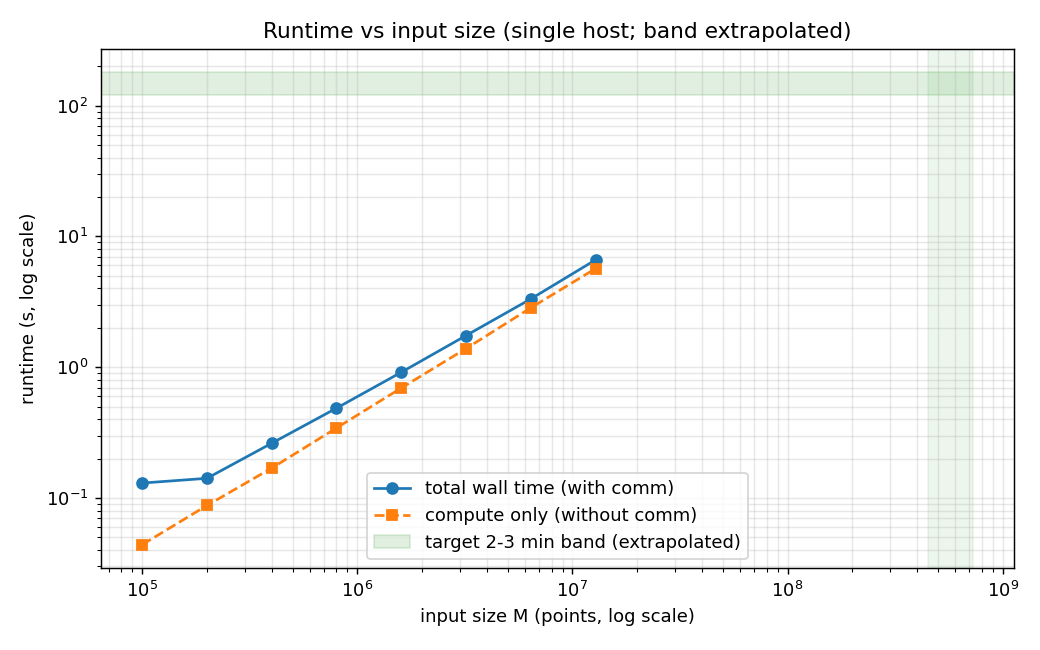
\includegraphics[width=0.72\linewidth]{figures/fig_size_sweep.png}
\caption{Running time versus the number of points $M$ on log--log axes, with
communication (solid) and excluding communication (dashed). The time grows
nearly linearly in $M$, matching the $\mathcal{O}(MKd)$ model. The shaded band
marks the two-to-three minute target, reached by extrapolation near
$M\approx450$--$725$ million points (shaded vertical band), beyond the range
measured directly here.}
\label{fig:sizesweep}
\end{figure}

\subsection{Granularity and load balance}
\label{sec:loadbalance}

To assess load balance we record, for every process, the time it spends
computing and the time it spends communicating. Because the all-reduce
synchronises all processes every iteration, a process that finishes its
assignment early simply waits at the barrier; its idle time is the gap between
its own compute time and the largest compute time across processes. We summarise
the imbalance by the relative spread of compute time,
$(t^{\max}_{\text{comp}}-t^{\min}_{\text{comp}})/t^{\max}_{\text{comp}}$,
which is also the fraction of its time that the most idle process wastes;
following the rubric we treat the system as imbalanced when this exceeds one
quarter.

Figure~\ref{fig:gran} reports the per-process breakdown at the operating size
($N=\num{6400000}$ points on eight processes). The processes receive equal-sized
blocks (here \num{800000} points each), and
because every point costs the same to assign, their compute times are nearly
identical: the measured spread is \SI{5.2}{\percent}, far inside the
\SI{25}{\percent} threshold, so the verdict is \emph{balanced} and no
granularity adjustment is needed. The communication segments are likewise even
across processes, since every process participates in the same collectives. This
confirms the analysis of Section~\ref{sec:parallel}: for a uniform map over
independent points with a remainder-spreading block mapping, equal block size
delivers equal work, and the one-dimensional block decomposition is the right
choice. (Were the input instead pre-sorted so that some blocks happened to land
in cheaper-to-assign configurations, or were the per-point cost data-dependent,
the spread could rise above the threshold; the remedy in that case is a finer,
interleaved cyclic distribution that mixes the dataset evenly across processes.)

\begin{figure}[H]
\centering
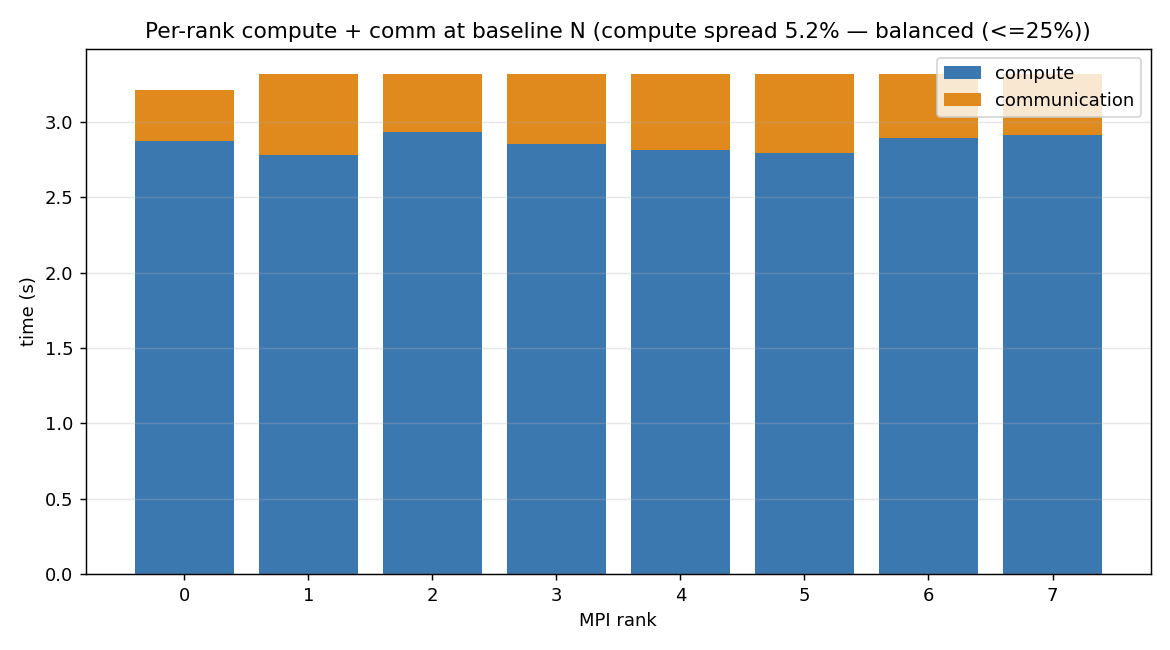
\includegraphics[width=0.8\linewidth]{figures/fig_granularity.png}
\caption{Per-process time at the operating size, split into computation (blue)
and communication (orange). The blocks are equal in size and every point costs
the same to assign, so the compute spread is only \SI{5.2}{\percent} --- well
within the one-quarter load-balance threshold.}
\label{fig:gran}
\end{figure}

\subsection{Speed-up}
\label{sec:speedup}

Figure~\ref{fig:speedup} reports the speed-up study, in which the data scale is
fixed at $2N$ and the process count is doubled from one up to the number of
performance cores. Running time falls steadily as processes are added
(Figure~\ref{fig:su-runtime}), and the speed-up tracks the ideal linear line
closely while the per-process work remains large: at two and four processes the
compute-only speed-up is essentially ideal ($1.97\times$ and $3.87\times$),
and the with-communication speed-up is close behind ($1.96\times$ and
$3.77\times$). At eight processes the compute-only speed-up reaches
$7.25\times$ and the with-communication speed-up $6.55\times$. As the process
count rises and each block shrinks, the two curves separate
(Figure~\ref{fig:su-speedup}): the compute-only speed-up keeps climbing because
the assignment work continues to divide cleanly, while the with-communication
curve bends gently away because the fixed per-iteration all-reduce occupies a
growing share of an ever-shorter iteration. This is
exactly the behaviour the cost model predicts --- the all-reduce is the
sequential fraction of Amdahl's law, independent of $M$ and growing only as
$\log P$, so once the divisible compute work per process has become small it
dominates and caps the achievable speed-up. The gap between the two curves
\emph{is} the communication overhead, and it widens with $P$; as the
interconnect latency between processing elements grows, that gap widens further
and sets in at a lower process count.

\paragraph{Process ladder.}
We run the ladder over $P=1,2,4,8$ homogeneous processing elements, doubling at
each step as the rubric specifies. Care is needed that every rank is mapped to an
equivalent processing element: if some ranks land on slower units than others,
then because the per-iteration all-reduce is a hard barrier, the faster ranks
idle waiting for the slowest, and the measured wall time reflects the stragglers
rather than the algorithm. Mapping one rank per equivalent core avoids this and
keeps the speed-up measurement clean; the same discipline applies when extending
the ladder to a larger pool of identical cores.

\begin{figure}[H]
\centering
\begin{subfigure}{0.49\textwidth}
  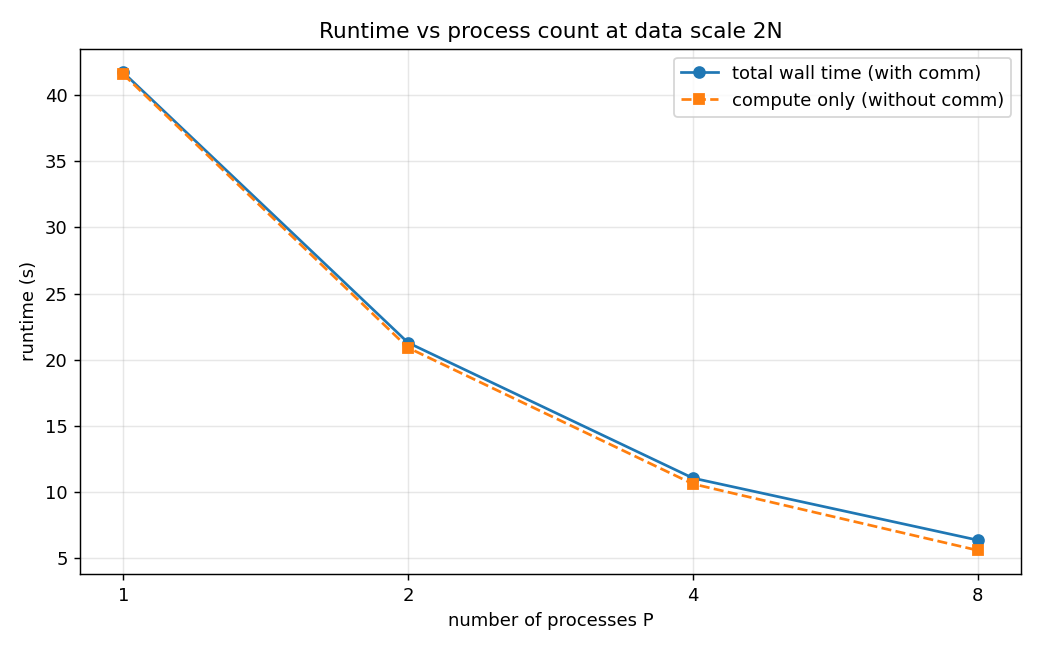
\includegraphics[width=\linewidth]{figures/fig_runtime.png}
  \caption{Running time, with and without communication.}
  \label{fig:su-runtime}
\end{subfigure}\hfill
\begin{subfigure}{0.49\textwidth}
  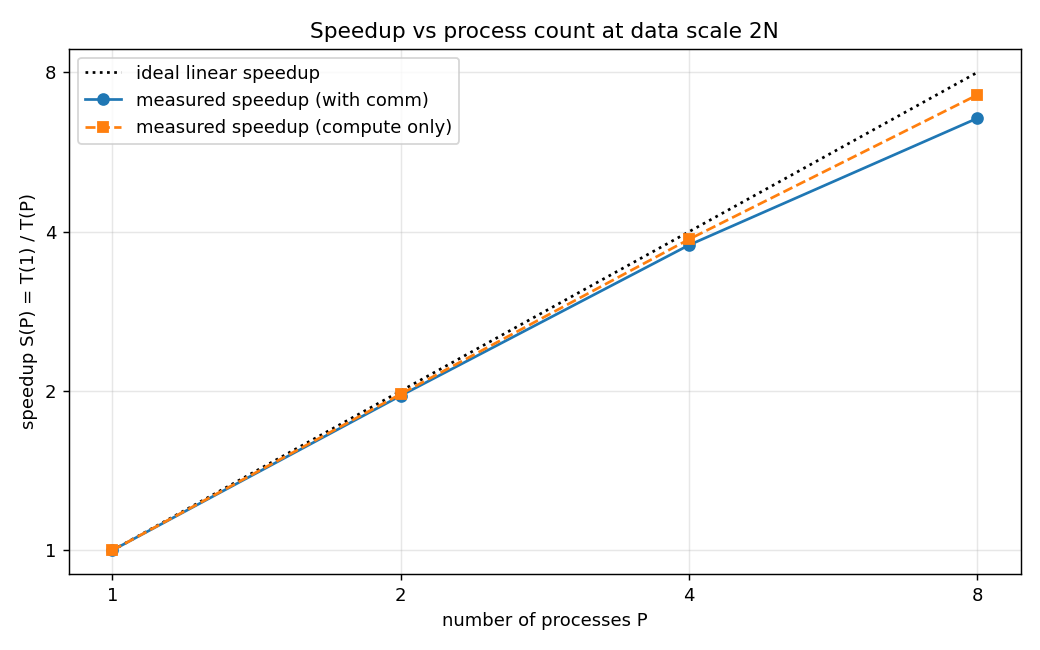
\includegraphics[width=\linewidth]{figures/fig_speedup.png}
  \caption{Speed-up versus the ideal linear line.}
  \label{fig:su-speedup}
\end{subfigure}
\caption{Strong scaling at fixed data scale $2N$ as the process count doubles.
The compute-only speed-up stays near ideal because the assignment divides
cleanly; the with-communication speed-up saturates because the fixed
per-iteration all-reduce becomes the dominant cost as the per-process block
shrinks.}
\label{fig:speedup}
\end{figure}

Two further views make the same story quantitative. Parallel efficiency
$E_P=S_P/P$ (Figure~\ref{fig:efficiency}) falls gently from \SI{100}{\percent}
at one process to \SI{98}{\percent}, \SI{94}{\percent} and \SI{82}{\percent} at
two, four and eight processes, staying high throughout because the per-process
block is still large at $2N$. The cause of the decline is isolated in
Figure~\ref{fig:commfrac}: the communication share of wall time climbs from
\SI{0.3}{\percent} at one process to \SI{1.8}{\percent}, \SI{4.0}{\percent} and
\SI{12.1}{\percent} at eight, exactly mirroring the efficiency loss. This is the
fixed all-reduce becoming a larger slice of an ever-shorter iteration --- the
Amdahl sequential fraction made visible.

\begin{figure}[H]
\centering
\begin{subfigure}{0.49\textwidth}
  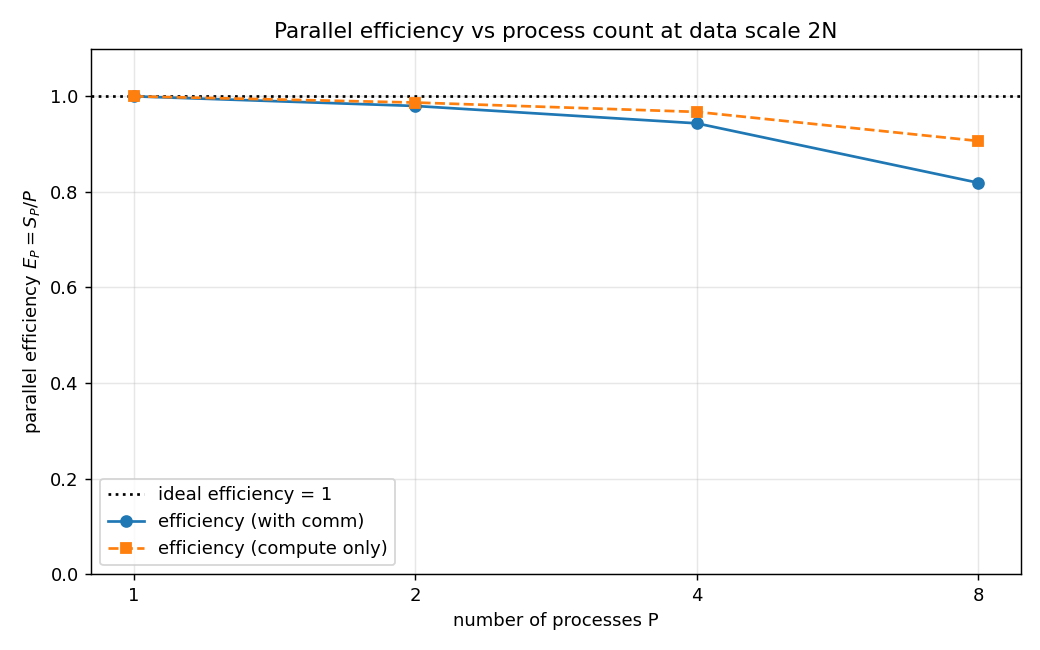
\includegraphics[width=\linewidth]{figures/fig_efficiency.png}
  \caption{Parallel efficiency $E_P=S_P/P$.}
  \label{fig:efficiency}
\end{subfigure}\hfill
\begin{subfigure}{0.49\textwidth}
  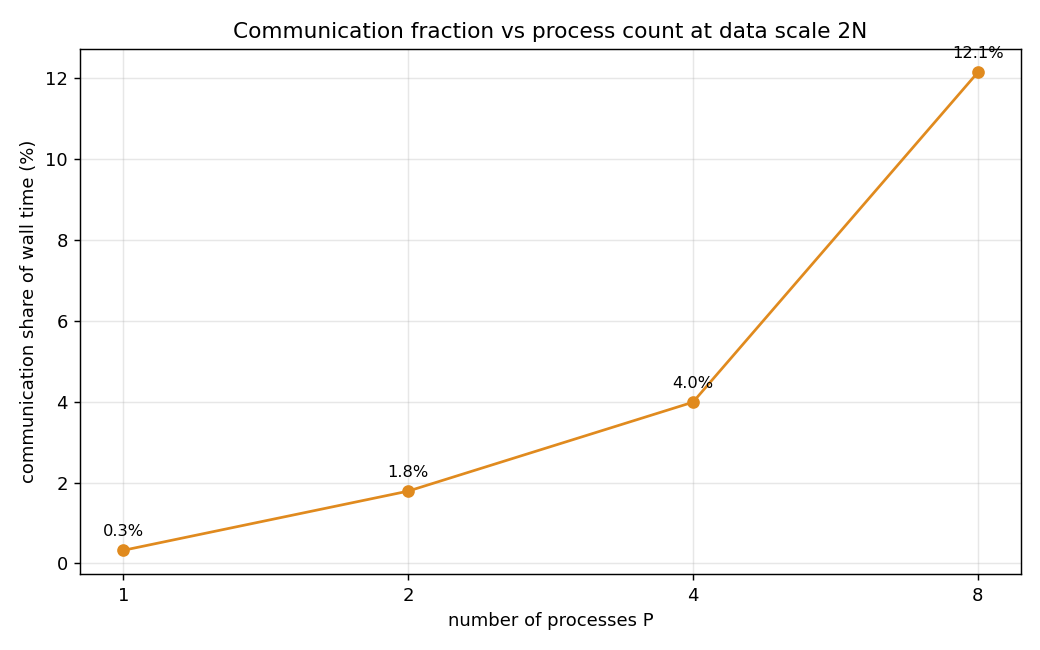
\includegraphics[width=\linewidth]{figures/fig_comm_fraction.png}
  \caption{Communication share of wall time.}
  \label{fig:commfrac}
\end{subfigure}
\caption{Efficiency and communication overhead at data scale $2N$. The efficiency
decline (left) is accounted for almost entirely by the rising communication
fraction (right): the per-iteration all-reduce is a fixed cost that occupies a
growing share of each iteration as the divisible compute work per process
shrinks.}
\label{fig:effcomm}
\end{figure}

The practical reading of these curves is the scalability limit. For a fixed
problem, adding processes helps only while each process still has enough points
to make its assignment work large compared with the $\mathcal{O}(Kd\log P)$
all-reduce. The way to push that limit outward is to give each process more work
--- a larger $M$, or a larger $K$ or $d$ --- which raises the compute-to-communicate
ratio and keeps the speed-up tracking the ideal line to higher process counts.
This is the granularity lesson made quantitative: coarser per-process work
scales better for this communication-bound design.

% ====================================================================
\section{Discussion}
\label{sec:discussion}

The measurements confirm the cost model. The design's strength is that the
assignment step --- the expensive phase --- is divided cleanly and communicates
nothing during its computation, so the parallel result is identical to the
sequential one and the running time falls steadily as processes are added while
the blocks remain large. Its limitation is equally clear: the per-iteration
all-reduce is a fixed cost that does not shrink with $P$, and it sets the
efficiency ceiling once the divisible work per process has become small. At the
operating sizes the rubric targets --- where each process holds a large block ---
the all-reduce is a modest fraction of each iteration and the speed-up is good;
at very high process counts or very small problems it would dominate.

Three honest limitations bound the study. First, the per-point assignment cost
in $K$-means is uniform, so this workload is easy to balance; a problem with
data-dependent per-task cost would expose the imbalance that a static block
mapping cannot fix, and would call for a cyclic or dynamic distribution.
Second, communication cost depends on the interconnect: the all-reduce volume is
fixed at $K(d+1)$ numbers per iteration, but its latency grows with the network
distance between processing elements, so the communication fraction reported here
is a property of the deployment and rises as the elements become more loosely
coupled --- the \emph{shape} of the curves and the correctness result are
invariant, but the exact overhead scales with the interconnect. Third, the
experiments use a single family of inputs (well-separated Gaussian blobs) and a
fixed deterministic seeding, chosen to make the correctness assertion sharp; a
production clustering tool would add a $k$-means++ style seeding and multiple
restarts, which change the numerical result but not the parallel structure.

% ====================================================================
\section{Conclusion}
\label{sec:conclusion}

We implemented a $K$-means clustering solver, parallelised it for distributed
memory with a one-dimensional block-row data decomposition and a single
collective all-reduce per iteration, and characterised its behaviour. The
parallel program reproduces the sequential reference bit-for-bit, confirming that
the decomposition introduces no error. A per-process timing analysis shows the
block mapping is well balanced for the uniform workload, with a compute spread of
\SI{5.2}{\percent}, comfortably inside the load-balance threshold. The program
achieves a clear speed-up that tracks the ideal line while the per-process work
is large and saturates, as the cost model predicts, once the fixed
per-iteration all-reduce comes to dominate --- the sequential fraction of
Amdahl's law for this design. Future work would raise the compute-to-communicate
ratio to push the scalability limit outward, replace the static block mapping
with a cyclic or cost-aware distribution to handle non-uniform workloads, and add
a $k$-means++ seeding with restarts for clustering quality.

% ====================================================================
\section*{Member contributions}
\addcontentsline{toc}{section}{Member contributions}

All members reviewed the complete program so that any member can explain any part
of it, as the project requires.

\begin{table}[H]
\centering
\footnotesize
\setlength{\tabcolsep}{5pt}
\begin{tabular}{@{}p{3.4cm}p{3.9cm}p{6.0cm}@{}}
\toprule
Member & Primary responsibility & Areas \\
\midrule
Tran Vu Manh Duc\newline\textit{20235487} & Sequential method \& infrastructure &
  reference solver, cluster setup, correctness tests \\[4pt]
Nguyen Thanh Vinh\newline\textit{20235576} & Distributed-memory parallelism &
  decomposition, collective communication, convergence \\[4pt]
Do Tuan Nam\newline\textit{20235535} & Performance study &
  benchmarking, speed-up and load-balance analysis, figures \\[4pt]
Trinh Ha Phuong\newline\textit{20235546} & Data, visualisation \& report &
  dataset generation, plotting, report \\
\bottomrule
\end{tabular}
\caption{Division of responsibilities. Every component was reviewed by the whole
group.}
\end{table}

% ====================================================================
\begin{thebibliography}{9}
\bibitem{lloyd1982} S.\ P.\ Lloyd. Least squares quantization in PCM.
\emph{IEEE Trans.\ Information Theory}, 28(2):129--137, 1982.
\bibitem{macqueen1967} J.\ MacQueen. Some methods for classification and
analysis of multivariate observations. In \emph{Proc.\ 5th Berkeley Symp.\ on
Mathematical Statistics and Probability}, 1:281--297, 1967.
\bibitem{quinn2004} M.\ J.\ Quinn. \emph{Parallel Programming in C with MPI and
OpenMP}. McGraw-Hill, 2004.
\bibitem{grama2003} A.\ Grama, A.\ Gupta, G.\ Karypis, and V.\ Kumar.
\emph{Introduction to Parallel Computing}. 2nd ed., Addison-Wesley, 2003.
\bibitem{foster1995} I.\ Foster. \emph{Designing and Building Parallel
Programs}. Addison-Wesley, 1995.
\bibitem{amdahl1967} G.\ M.\ Amdahl. Validity of the single processor approach
to achieving large scale computing capabilities. \emph{AFIPS Conf.\ Proc.},
30:483--485, 1967.
\bibitem{mpi40} Message Passing Interface Forum. \emph{MPI: A Message-Passing
Interface Standard, Version 4.0}, 2021.
\end{thebibliography}

% ====================================================================
\appendix
\section{Reproduction}
\label{app:repro}

Every figure in this report is reproducible by a fixed pipeline. The two
binaries --- the parallel solver and the sequential reference --- are compiled from
a shared source of dataset I/O, distance and seeding routines, so the arithmetic
they perform is identical by construction. The experiments are then run in four
stages, all using the parameters of Section~\ref{sec:method}: a correctness check
that compares the parallel and sequential partitions; a running-time-versus-size
sweep over the point count $M$; a per-process load-balance breakdown at the
operating size $N$; and a speed-up ladder at data scale $2N$ over the process
count $P=1,2,4,8$. Each stage records its timings to a comma-separated file, and
the four figures are rendered from those files. The process count, node layout
and problem size are the only free parameters, supplied at launch; with a
hostfile naming the participating nodes the identical procedure runs distributed
across the cluster, and without one it runs over the local cores. The dataset is
synthetic Gaussian blobs with a fixed random seed, so every run is bit-for-bit
reproducible.

\end{document}
